\documentclass[aspectratio=169,11pt]{beamer}
\usepackage[T1]{fontenc}
\usepackage[utf8]{inputenc}
\usepackage{lmodern,amsmath,amssymb,graphicx,tikz}
\usetikzlibrary{arrows.meta,calc}
\usetheme{default}
\usefonttheme{serif}
\setbeamercolor{normal text}{fg=black,bg=white}
\setbeamercolor{structure}{fg=black}
\setbeamercolor{frametitle}{fg=black}
\setbeamercolor{title}{fg=black}
\setbeamertemplate{navigation symbols}{}
\setbeamertemplate{footline}[frame number]
\setbeamertemplate{itemize items}[circle]
\setbeamersize{text margin left=8mm,text margin right=8mm}
\setlength{\parskip}{5pt}
\newcommand{\cO}{\mathcal O}
\newcommand{\cI}{\mathcal I}
\newcommand{\cA}{\mathcal A}
\newcommand{\db}{\bar\partial}
\newcommand{\C}{\mathbb C}
\newcommand{\Pj}{\mathbb P}
\newcommand{\norm}[1]{\lVert#1\rVert}
\newcommand{\src}[1]{\par\vfill{\scriptsize #1\par}}
\author{Daniel Gonz\'alez Casanova Azuela}

\title{Positive curvature gives coordinates}
\subtitle{Kodaira's embedding theorem}
\date{5 November 2026}
\begin{document}
\begin{frame}\titlepage\end{frame}

% ------------------------------------------------------------------
% Main talk (about nine minutes)
% ------------------------------------------------------------------

\begin{frame}{The plan}
\begin{enumerate}
\setlength{\itemsep}{16pt}
\item Projective space carries a \textbf{positive} form: Fubini--Study.
\item Kodaira's theorem is the \textbf{converse}.
\item The proof: sections, three conditions, and \textbf{harmonic forms}.
\end{enumerate}
\end{frame}

\begin{frame}{Projective space has a positive form}
A point of \(\Pj^n\) is a line in \(\C^{n+1}\): \([z_0:\cdots:z_n]=[\lambda z_0:\cdots:\lambda z_n]\).
\par\medskip
In the chart \(z_0=1\), the \textbf{Fubini--Study form} is
\[
\omega_{\rm FS}=\frac{i}{2\pi}\,\partial\db\log\bigl(1+|z|^2\bigr).
\]
On a tangent vector \(v\neq0\), up to a positive factor, it gives
\[
\frac{(1+|z|^2)|v|^2-|\langle z,v\rangle|^2}{(1+|z|^2)^2}
\ \ge\ \frac{|v|^2}{(1+|z|^2)^2}\ >\ 0 .
\]
The inequality is Cauchy--Schwarz. So \(\omega_{\rm FS}\) is \textbf{positive}.
\src{Fubini (1904), Study (1905). \(\omega_{\rm FS}\) is the curvature form of the line bundle \(\cO(1)\).}
\end{frame}

\begin{frame}{Positivity passes to submanifolds}
Let \(X\subset\Pj^N\) be a compact complex submanifold.
\par\bigskip
Restrict the line bundle: \(L=\cO(1)|_X\).
\par\medskip
Its curvature is \(\omega_{\rm FS}|_X\), and it is still positive.
\par\bigskip
\begin{center}
\Large\(X\) projective \(\ \Longrightarrow\ \) \(X\) has a positive line bundle.
\end{center}
\par\bigskip
Question: is the converse true?
\end{frame}

\begin{frame}{Kodaira embedding theorem (1954)}
Let \(X\) be a compact complex manifold and \(L\) a holomorphic line bundle
with a metric of \textbf{positive curvature}.
\par\medskip
Then, for large \(k\), the sections of \(L^{\otimes k}\) give an embedding
\[
\boxed{\Phi:X\hookrightarrow\Pj^N.}
\]
\par\medskip
\begin{center}
\Large Positive \(\ \Longrightarrow\ \) projective.
\end{center}
\src{K. Kodaira, Ann. of Math. 60 (1954), 28--48.}
\end{frame}

\begin{frame}{Kunihiko Kodaira (1915--1997)}
\begin{columns}[c]
\column{.36\textwidth}
\centering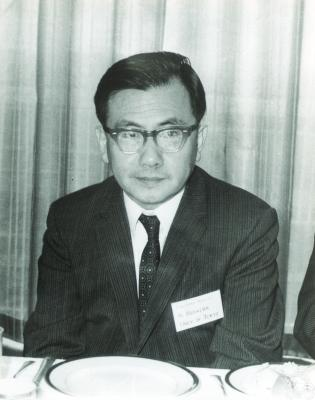
\includegraphics[height=4.8cm]{../assets/Kunihiko_Kodaira.png}
\column{.59\textwidth}
Fields Medal, 1954.
\par\bigskip
His idea: an \textbf{analytic} condition (curvature)
produces an \textbf{algebraic} object (polynomial equations).
\end{columns}
\src{Photo: Konrad Jacobs / MFO, Tokyo 1969, CC BY-SA 2.0 DE. Historical source: IAS scholar profile.}
\end{frame}

\begin{frame}{Where this sits in history}
\begin{center}
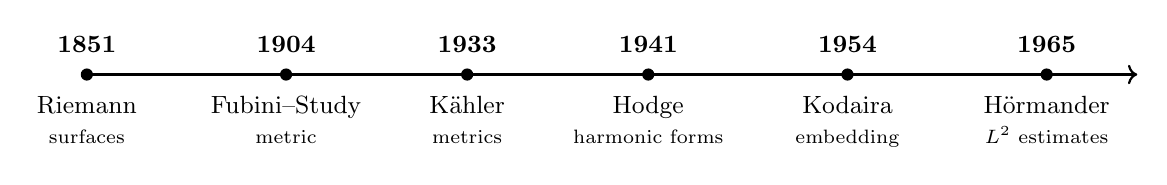
\begin{tikzpicture}[x=1.15cm]
\draw[thick,->] (0,0)--(11.6,0);
\foreach \x/\y/\t/\s in {
 0/1851/Riemann/surfaces,
 2.2/1904/Fubini--Study/metric,
 4.2/1933/Kähler/metrics,
 6.2/1941/Hodge/harmonic forms,
 8.4/1954/Kodaira/embedding,
 10.6/1965/Hörmander/\(L^2\) estimates}
{\fill (\x,0) circle (2.2pt);
 \node[above] at (\x,.15) {\small\textbf{\y}};
 \node[below,align=center] at (\x,-.15) {\small \t\\[-1pt]\scriptsize\s};}
\end{tikzpicture}
\end{center}
\par\bigskip
One theme: \textbf{analysis produces functions}.
\par\medskip
Riemann used analysis to prove that compact Riemann surfaces are algebraic curves.
Kodaira did the same in every dimension.
\src{More history in the appendix.}
\end{frame}

\begin{frame}{Sections give a map}
Choose a basis \(s_0,\ldots,s_m\) of the holomorphic sections of \(L\).
\par\medskip
In a local frame \(e\), write \(s_j=f_j\,e\). Define the \textbf{canonical map}
\[
\Phi_L(x)=[f_0(x):\cdots:f_m(x)]\in\Pj^m.
\]
\par\medskip
A new frame multiplies every \(f_j\) by the same number.
\par\smallskip
So the point of \(\Pj^m\) does not change.
\end{frame}

\begin{frame}{Three conditions}
\begin{center}
\renewcommand{\arraystretch}{1.9}
\begin{tabular}{ll}
The sections \(\ldots\) & The map \(\Phi_L\) is \(\ldots\)\\\hline
have no common zero (\textbf{base-point free}) & defined everywhere\\
\textbf{separate points} & injective\\
\textbf{separate tangent directions} & an immersion
\end{tabular}
\end{center}
\par\bigskip
On a compact manifold, an injective immersion is an embedding.
\end{frame}

\begin{frame}{Each condition is a lifting problem}
We want global sections with \textbf{prescribed values} at \(x\) and \(y\),
or prescribed \textbf{first derivatives} at \(x\).
\par\medskip
An exact sequence gives
\[
H^0(X,L^k)\ \longrightarrow\ \text{prescribed data}\ \longrightarrow\ H^1(X,\,\cdots).
\]
\[
\boxed{H^1=0\quad\Longrightarrow\quad\text{every choice of data lifts.}}
\]
After blowing up \(x\) and \(y\), this \(H^1\) has the form
\(H^1(K\otimes B)\), with \(B\) positive when \(k\) is large.
\src{A sketch: the blow-up step is not shown. See Griffiths--Harris, Ch.~1 \S4.}
\end{frame}

\begin{frame}{Hodge theory: one harmonic form per class}
On a compact Kähler manifold, every class in
\[
H^q(X,K_X\otimes B)
\]
has exactly one \textbf{harmonic} representative \(u\):
\[
\Delta u=0,\qquad\text{equivalently}\quad \db u=0\ \text{and}\ \db^*u=0.
\]
\par\bigskip
\begin{center}
\large To prove \(H^q=0\), show that every harmonic form is zero.
\end{center}
\end{frame}

\begin{frame}{Bochner--Kodaira: harmonic forms must vanish}
The Bochner--Kodaira formula compares two Laplacians:
\[
\Delta_{\db}=\Delta_{\partial}+[\,i\Theta_B,\Lambda\,].
\]
If \(i\Theta_B\ge\varepsilon\omega\), the curvature term is at least \(q\varepsilon\) on \((n,q)\)-forms.
\par\medskip
Integrate against a harmonic \(u\):
\[
0=\underbrace{\norm{\partial u}^2+\norm{\partial^*u}^2}_{\ge0}
+\underbrace{\langle[i\Theta_B,\Lambda]u,u\rangle}_{\ge q\varepsilon\norm u^2}.
\]
For \(q>0\), this forces \(u=0\). So \(\boxed{H^q(X,K_X\otimes B)=0.}\)
\src{Kodaira vanishing: Kodaira, Proc.\ Nat.\ Acad.\ Sci.\ 39 (1953), after Bochner (1946).}
\end{frame}

\begin{frame}{Summary}
\begin{center}
\renewcommand{\arraystretch}{1.5}
\begin{tabular}{c}
positive curvature\\
\(\Downarrow\) \small Bochner--Kodaira\\
no harmonic forms, so \(H^1=0\)\\
\(\Downarrow\) \small exact sequence\\
enough sections: the three conditions\\
\(\Downarrow\)\\
an embedding \(X\hookrightarrow\Pj^N\)
\end{tabular}
\end{center}
\par\medskip
\centering\large Thank you.
\end{frame}

% ------------------------------------------------------------------
% Appendix: history (not part of the timed talk)
% ------------------------------------------------------------------

\begin{frame}
\centering\Large Appendix\par\bigskip
\large A short history of complex and Kähler geometry
\end{frame}

\begin{frame}{Overview}
\begin{center}
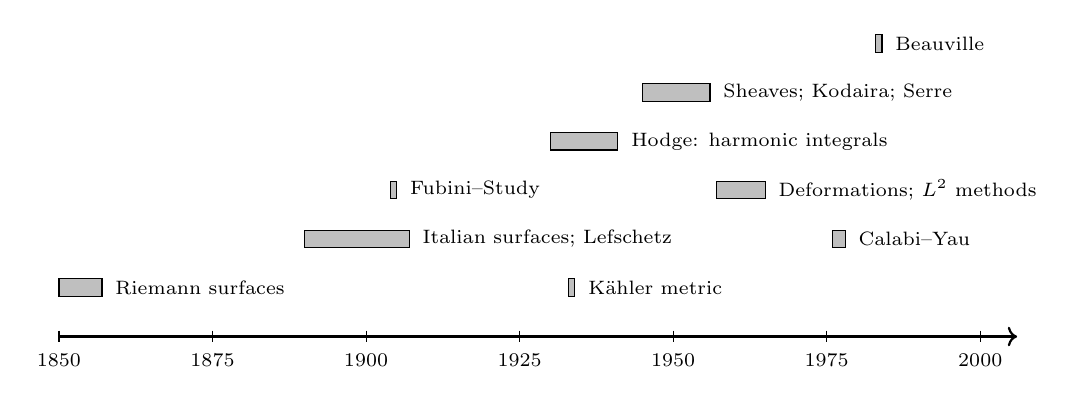
\begin{tikzpicture}[x=.078cm,y=.62cm]
\draw[thick,->] (0,0)--(156,0);
\foreach \x in {0,25,50,75,100,125,150}
 {\draw (\x,.12)--(\x,-.12); \node[below] at (\x,-.15) {\scriptsize\the\numexpr1850+\x\relax};}
\foreach \a/\b/\h/\t in {
 0/7/1/Riemann surfaces,
 40/57/2/Italian surfaces; Lefschetz,
 54/55/3/Fubini--Study,
 83/84/1/Kähler metric,
 80/91/4/Hodge: harmonic integrals,
 95/106/5/Sheaves; Kodaira; Serre,
 107/115/3/Deformations; \(L^2\) methods,
 126/128/2/Calabi--Yau,
 133/134/6/Beauville}
{\fill[black!25] (\a,\h-.18) rectangle (\b,\h+.18);
 \draw (\a,\h-.18) rectangle (\b,\h+.18);
 \node[right] at (\b+.6,\h) {\scriptsize\t};}
\end{tikzpicture}
\end{center}
\src{Dates refer to the main publications cited on the following slides.}
\end{frame}

\begin{frame}{1851--1913: Riemann surfaces}
\begin{itemize}
\setlength{\itemsep}{10pt}
\item \textbf{Riemann} (dissertation 1851; \emph{Abelian functions} 1857)
introduced Riemann surfaces to study many-valued functions.
\item He used the \textbf{Dirichlet principle} (minimizing an energy)
to construct functions. Conclusion: compact Riemann surfaces are algebraic curves.
\item Weierstrass criticized the Dirichlet principle.
Hilbert repaired it around 1900; Weyl gave the modern definition of a Riemann surface (1913).
\end{itemize}
\par\medskip
\textbf{The first instance of our theme:} analysis produces functions,
and functions produce an algebraic curve.
\src{Riemann, Crelle 54 (1857); Weyl, \emph{Die Idee der Riemannschen Fläche} (1913).}
\end{frame}

\begin{frame}{1880--1930: more variables and topology}
\begin{itemize}
\setlength{\itemsep}{10pt}
\item \textbf{Algebraic surfaces:} Picard, Castelnuovo and Enriques
classify surfaces with algebraic and geometric methods.
\item \textbf{Several complex variables are different:}
Hartogs (1906) shows that holomorphic functions extend across holes;
Poincaré (1907) shows that the ball and the bidisc are not biholomorphic.
\item \textbf{Topology:} Lefschetz (1924), \emph{L'analysis situs et la géométrie algébrique}.
In his words, he planted
``the harpoon of algebraic topology into the body of the whale of algebraic geometry.''
\end{itemize}
\src{Lefschetz, ``A page of mathematical autobiography'', Bull.\ AMS 74 (1968).}
\end{frame}

\begin{frame}{1904--1933: metrics}
\begin{itemize}
\setlength{\itemsep}{12pt}
\item \textbf{Fubini} (1904) and \textbf{Study} (1905) studied the natural
Hermitian metric of projective space.
\item \textbf{Kähler} (1933), \emph{Über eine bemerkenswerte Hermitesche Metrik}:
Hermitian metrics with \(d\omega=0\).
\item He noticed that such metrics come from a local potential:
\[
\omega=i\,\partial\db\varphi .
\]
Fubini--Study is the example with \(\varphi=\log(1+|z|^2)\), up to a constant.
\end{itemize}
\src{Fubini, Atti Ist.\ Veneto 63 (1904); Study, Math.\ Ann.\ 60 (1905);
Kähler, Abh.\ Math.\ Sem.\ Hamburg 9 (1933), 173--186.}
\end{frame}

\begin{frame}{1930--1950: harmonic integrals}
\begin{itemize}
\setlength{\itemsep}{10pt}
\item \textbf{Hodge}: every cohomology class has a harmonic representative.
Book: \emph{The theory and applications of harmonic integrals} (1941).
\item On Kähler manifolds, harmonic forms split by type: the \textbf{Hodge decomposition}
\(H^k=\bigoplus_{p+q=k}H^{p,q}\).
\item The analysis had a gap; \textbf{Weyl} (1943) and \textbf{Kodaira} (1949) supplied proofs.
\item Hodge's 1950 ICM address: which classes come from subvarieties?
This became the \textbf{Hodge conjecture}.
\end{itemize}
\par\medskip
Kähler's condition is exactly what makes Hodge's theory work well.
\src{Weyl, Ann.\ of Math.\ 44 (1943), 1--6; Kodaira, Ann.\ of Math.\ 50 (1949).}
\end{frame}

\begin{frame}{1945--1956: sheaves and characteristic classes}
\begin{itemize}
\setlength{\itemsep}{10pt}
\item \textbf{Leray} invents sheaves; the \textbf{Cartan} seminar makes them a tool of complex analysis.
\item \textbf{Chern} (1946): characteristic classes of Hermitian bundles, from curvature.
\item \textbf{Dolbeault} (1953): \(\db\)-cohomology computes sheaf cohomology.
\item \textbf{Chow} (1949): closed analytic subsets of \(\Pj^N\) are algebraic.
\textbf{Serre}, GAGA (1956): analytic and algebraic geometry agree on projective varieties.
\end{itemize}
\par\medskip
With Kodaira: a positive line bundle makes \(X\) an \emph{algebraic} variety.
\src{Chow, Amer.\ J.\ Math.\ 71 (1949); Dolbeault, C.\ R.\ Acad.\ Sci.\ 236 (1953);
Serre, Ann.\ Inst.\ Fourier 6 (1956).}
\end{frame}

\begin{frame}{1953--1954: Kodaira's decisive years}
\begin{itemize}
\setlength{\itemsep}{10pt}
\item \textbf{Bochner} (1946): curvature forbids certain harmonic objects.
\item \textbf{Kodaira} (1953): the same method gives the vanishing theorem.
\item \textbf{Kodaira} (1954): the embedding theorem. A compact Kähler manifold
whose Kähler class is \emph{integral} is projective.
\item \textbf{Hirzebruch} (1954): Riemann--Roch in every dimension.
\item Fields Medals 1954: \textbf{Kodaira} and \textbf{Serre}.
\end{itemize}
\src{Bochner, Bull.\ AMS 52 (1946), 776--797; Kodaira, PNAS 39 (1953), 1268--1273;
Kodaira, Ann.\ of Math.\ 60 (1954), 28--48.}
\end{frame}

\begin{frame}{1957--2004: Kähler is not projective}
\begin{itemize}
\setlength{\itemsep}{10pt}
\item \textbf{Newlander--Nirenberg} (1957): integrable almost complex structures are complex.
\item \textbf{Kodaira--Spencer} (1958): deformations of complex structures.
\item Kodaira's surface classification: every compact Kähler surface
deforms to a projective one.
\item \textbf{Voisin} (2004): in dimension \(\ge4\), some compact Kähler manifolds
do not even have the homotopy type of a projective manifold.
\end{itemize}
\par\medskip
So Kodaira's theorem draws a real boundary inside Kähler geometry.
\src{Voisin, Invent.\ Math.\ 157 (2004), 329--343.}
\end{frame}

\begin{frame}{1954--2015: analysis takes over}
\begin{itemize}
\setlength{\itemsep}{10pt}
\item \textbf{Hörmander} (1965), Andreotti--Vesentini (1965):
\(L^2\) estimates for \(\db\). Kodaira's method, made flexible.
\item \textbf{Calabi} (1954, 1957) conjectured Ricci-flat Kähler metrics;
\textbf{Yau} proved it (1977, 1978). Aubin and Yau treated the negative case.
\item \textbf{Nadel} (1990) and \textbf{Demailly}: multiplier ideals,
vanishing with singular metrics.
\item \textbf{Chen--Donaldson--Sun} (2015): Kähler--Einstein metrics on Fano manifolds
and K-stability.
\end{itemize}
\src{Hörmander, Acta Math.\ 113 (1965); Yau, PNAS 74 (1977), CPAM 31 (1978);
Chen--Donaldson--Sun, J.\ AMS 28 (2015).}
\end{frame}

\begin{frame}{Where hyperkähler geometry enters}
\begin{itemize}
\setlength{\itemsep}{10pt}
\item Calabi--Yau (1978) gives Ricci-flat metrics; holonomy \(\operatorname{Sp}(n)\) gives
\textbf{hyperkähler} manifolds.
\item \textbf{Beauville} (1983): \(S^{[n]}\), generalized Kummers, and the form \(q_X\) on \(H^2\).
\item \textbf{Huybrechts} (1999; erratum 2003): \(X\) is projective iff some line bundle has \(q_X(L)>0\).
\end{itemize}
\par\medskip
\begin{center}
\renewcommand{\arraystretch}{1.4}
\begin{tabular}{ll}
Kodaira: & a positive \emph{form} \(\Rightarrow\) an embedding\\
Huybrechts: & a positive \emph{number} \(q_X(L)\) \(\Rightarrow\) projective\\
SYZ (conjecture): & nef \(L\), \(q_X(L)=0\) \(\Rightarrow\) a Lagrangian fibration
\end{tabular}
\end{center}
\src{Beauville, J.\ Diff.\ Geom.\ 18 (1983); Huybrechts, Invent.\ Math.\ 135 (1999), 152 (2003).
See HP, \emph{Reading the masters}, Huybrechts section.}
\end{frame}

\begin{frame}{Further reading}
\begin{itemize}
\setlength{\itemsep}{8pt}
\item P.~Griffiths, J.~Harris, \emph{Principles of algebraic geometry} (1978), Ch.~0--1.
\item D.~Huybrechts, \emph{Complex geometry} (2005), Ch.~5.
\item C.~Voisin, \emph{Hodge theory and complex algebraic geometry I} (2002).
\item J.-P.~Demailly, \emph{Complex analytic and differential geometry}, Ch.~VII.
\item A.~Weil, \emph{Introduction à l'étude des variétés kählériennes} (1958).
\end{itemize}
\end{frame}
\end{document}
